\documentclass[12pt]{article}
%--------------------   start of the 'preamble'
%
\usepackage{graphicx,amssymb,amstext,amsmath,color}
\usepackage[margin=2cm]{geometry}
\usepackage{abstract}
\usepackage{setspace}
\usepackage[footnotesize,bf]{caption}

% TABLE
\usepackage{multicol,hhline,colortbl,multirow}
\usepackage{braket}
\usepackage{siunitx}
\usepackage{hyperref}
\usepackage{authblk}
\usepackage{siunitx}
\usepackage{mathrsfs}
%%\usepackage[sort&compress]{natbib}
%%\bibpunct{(}{)}{,}{a}{, }{;}
%
\usepackage[sort&compress]{natbib}
\bibpunct{[}{]}{,}{s}{}{;}


\definecolor{gray}{gray}{0.8}
\def\mobunits{\square\centi\meter\per\volt\per\second}
\def\gcm{\gram\per\cubic\centi\meter}
\def\ccg{\cellcolor{gray}}

\renewcommand{\labelitemii}{$\circ$}
\renewcommand{\bibname}{References}


\title{MorphCT Results - P3HT}
\author{Matthew Jones}
\date{\today}

\begin{document}
\maketitle

\section{Increasing Simulation Time, $\tau$}

\begin{center}
\begin{tabular}{| c | c | c | c | c | c | c |}
\hline
\rule{0pt}{2.5ex} 
\multirow{2}{*}{\textbf{ID}}&\multirow{2}{*}{\textbf{Simulation Name}}&\textbf{Density}&\textbf{Anisotropy}&\textbf{Anisotropy}&\textbf{Mobility}&\textbf{Intra-}\\
                            &&(\SI{}{\gcm})&(Arb. U.)&(Shape)&(\SI{}{\mobunits})&\textbf{\%}\\
\hhline{|=======|}
\textbf{\ccg1}&\rule{0pt}{2.5ex}\ccg 0001\_withImages&\ccg 1.061&\ccg 0.0038&\ccg Spherical&\ccg1.56$\times 10^{-1}$&\ccg27.04\%\\
\textbf{2}&\rule{0pt}{2.5ex}0005\_withImages&1.336&0.0046&Spherical&7.19$\times 10^{-3}$&21.27\%\\
\textbf{\ccg3}&\rule{0pt}{2.5ex}\ccg 0010\_withImages&\ccg 1.345&\ccg 0.0076&\ccg Spherical&\ccg2.41$\times 10^{-2}$&\ccg20.68\%\\
\textbf{4}&\rule{0pt}{2.5ex}0020\_withImages&1.428&0.0111&Spherical&1.09$\times 10^{-2}$&19.28\%\\
\textbf{\ccg5}&\rule{0pt}{2.5ex}\ccg 0040\_withImages&\ccg 1.450&\ccg 0.0114&\ccg Spherical&\ccg1.74$\times 10^{-2}$&\ccg18.75\%\\
\textbf{6}&\rule{0pt}{2.5ex}0100\_withImages&1.510&0.0216&Spherical&1.49$\times 10^{-2}$&15.66\%\\
\textbf{\ccg7}&\rule{0pt}{2.5ex}\ccg 0200\_withImages&\ccg 1.554&\ccg 0.1245&\ccg Ellipsoid&\ccg1.07$\times 10^{0}$&\ccg14.41\%\\
\textbf{8}&\rule{0pt}{2.5ex}0300\_withImages&1.593&0.2135&Disk&$5.73\times 10^{-1}$&13.75\%\\
\textbf{\ccg9}&\rule{0pt}{2.5ex}\ccg 0500\_withImages&\ccg 1.638&\ccg 0.2376&\ccg Disk&\ccg3.53$\times 10^{0}$&\ccg13.06\%\\
\textbf{10}&\rule{0pt}{2.5ex}1000\_withImages&1.662&0.2479&Disk&1.88$\times 10^{0}$&12.60\%\\
\hhline{-------}
\end{tabular}\label{table:mob}
\captionof{table}{The results from the new data given a snapshot of the pristine P3HT morphology at a given snapshot corresponding to simulation time, $\tau$.}
\end{center}

\begin{figure}[h!]\centering
	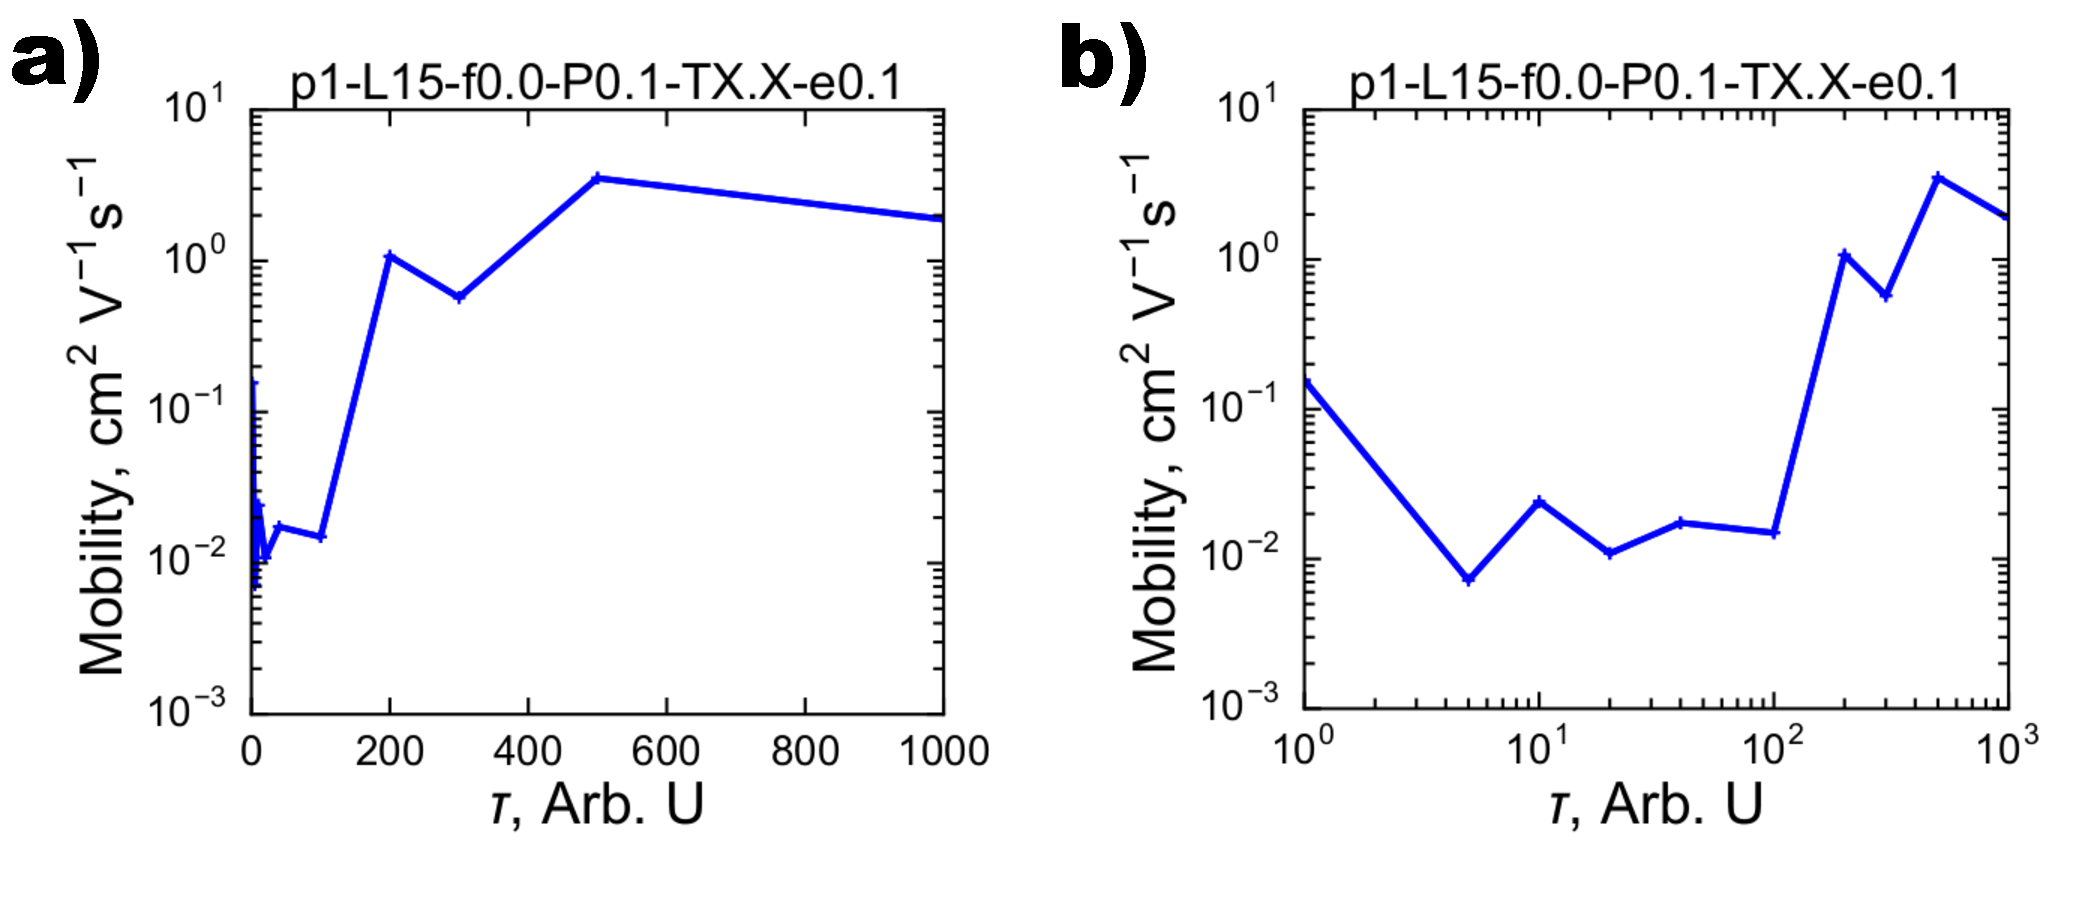
\includegraphics[width=\textwidth]{Figures/HoleMob.pdf}
    \caption{The mobility trend observed as a function of increasing dimensionless evolution time}
	\label{fig:MSD}
\end{figure}

Representative Values From Literature:
\begin{itemize}
    \item{Density: \SI{1.10}{\gcm}\cite{Newbloom2012a}}
\item{Mobility: \SI{1E-5}{} - \SI{1E-3}{\mobunits}\cite{Ballantyne2008b,Mauer2010,Pandey2000,Kim2006}}
\end{itemize}

\clearpage

\subsection{3D Carrier Network}

\begin{figure}[h!]\centering
	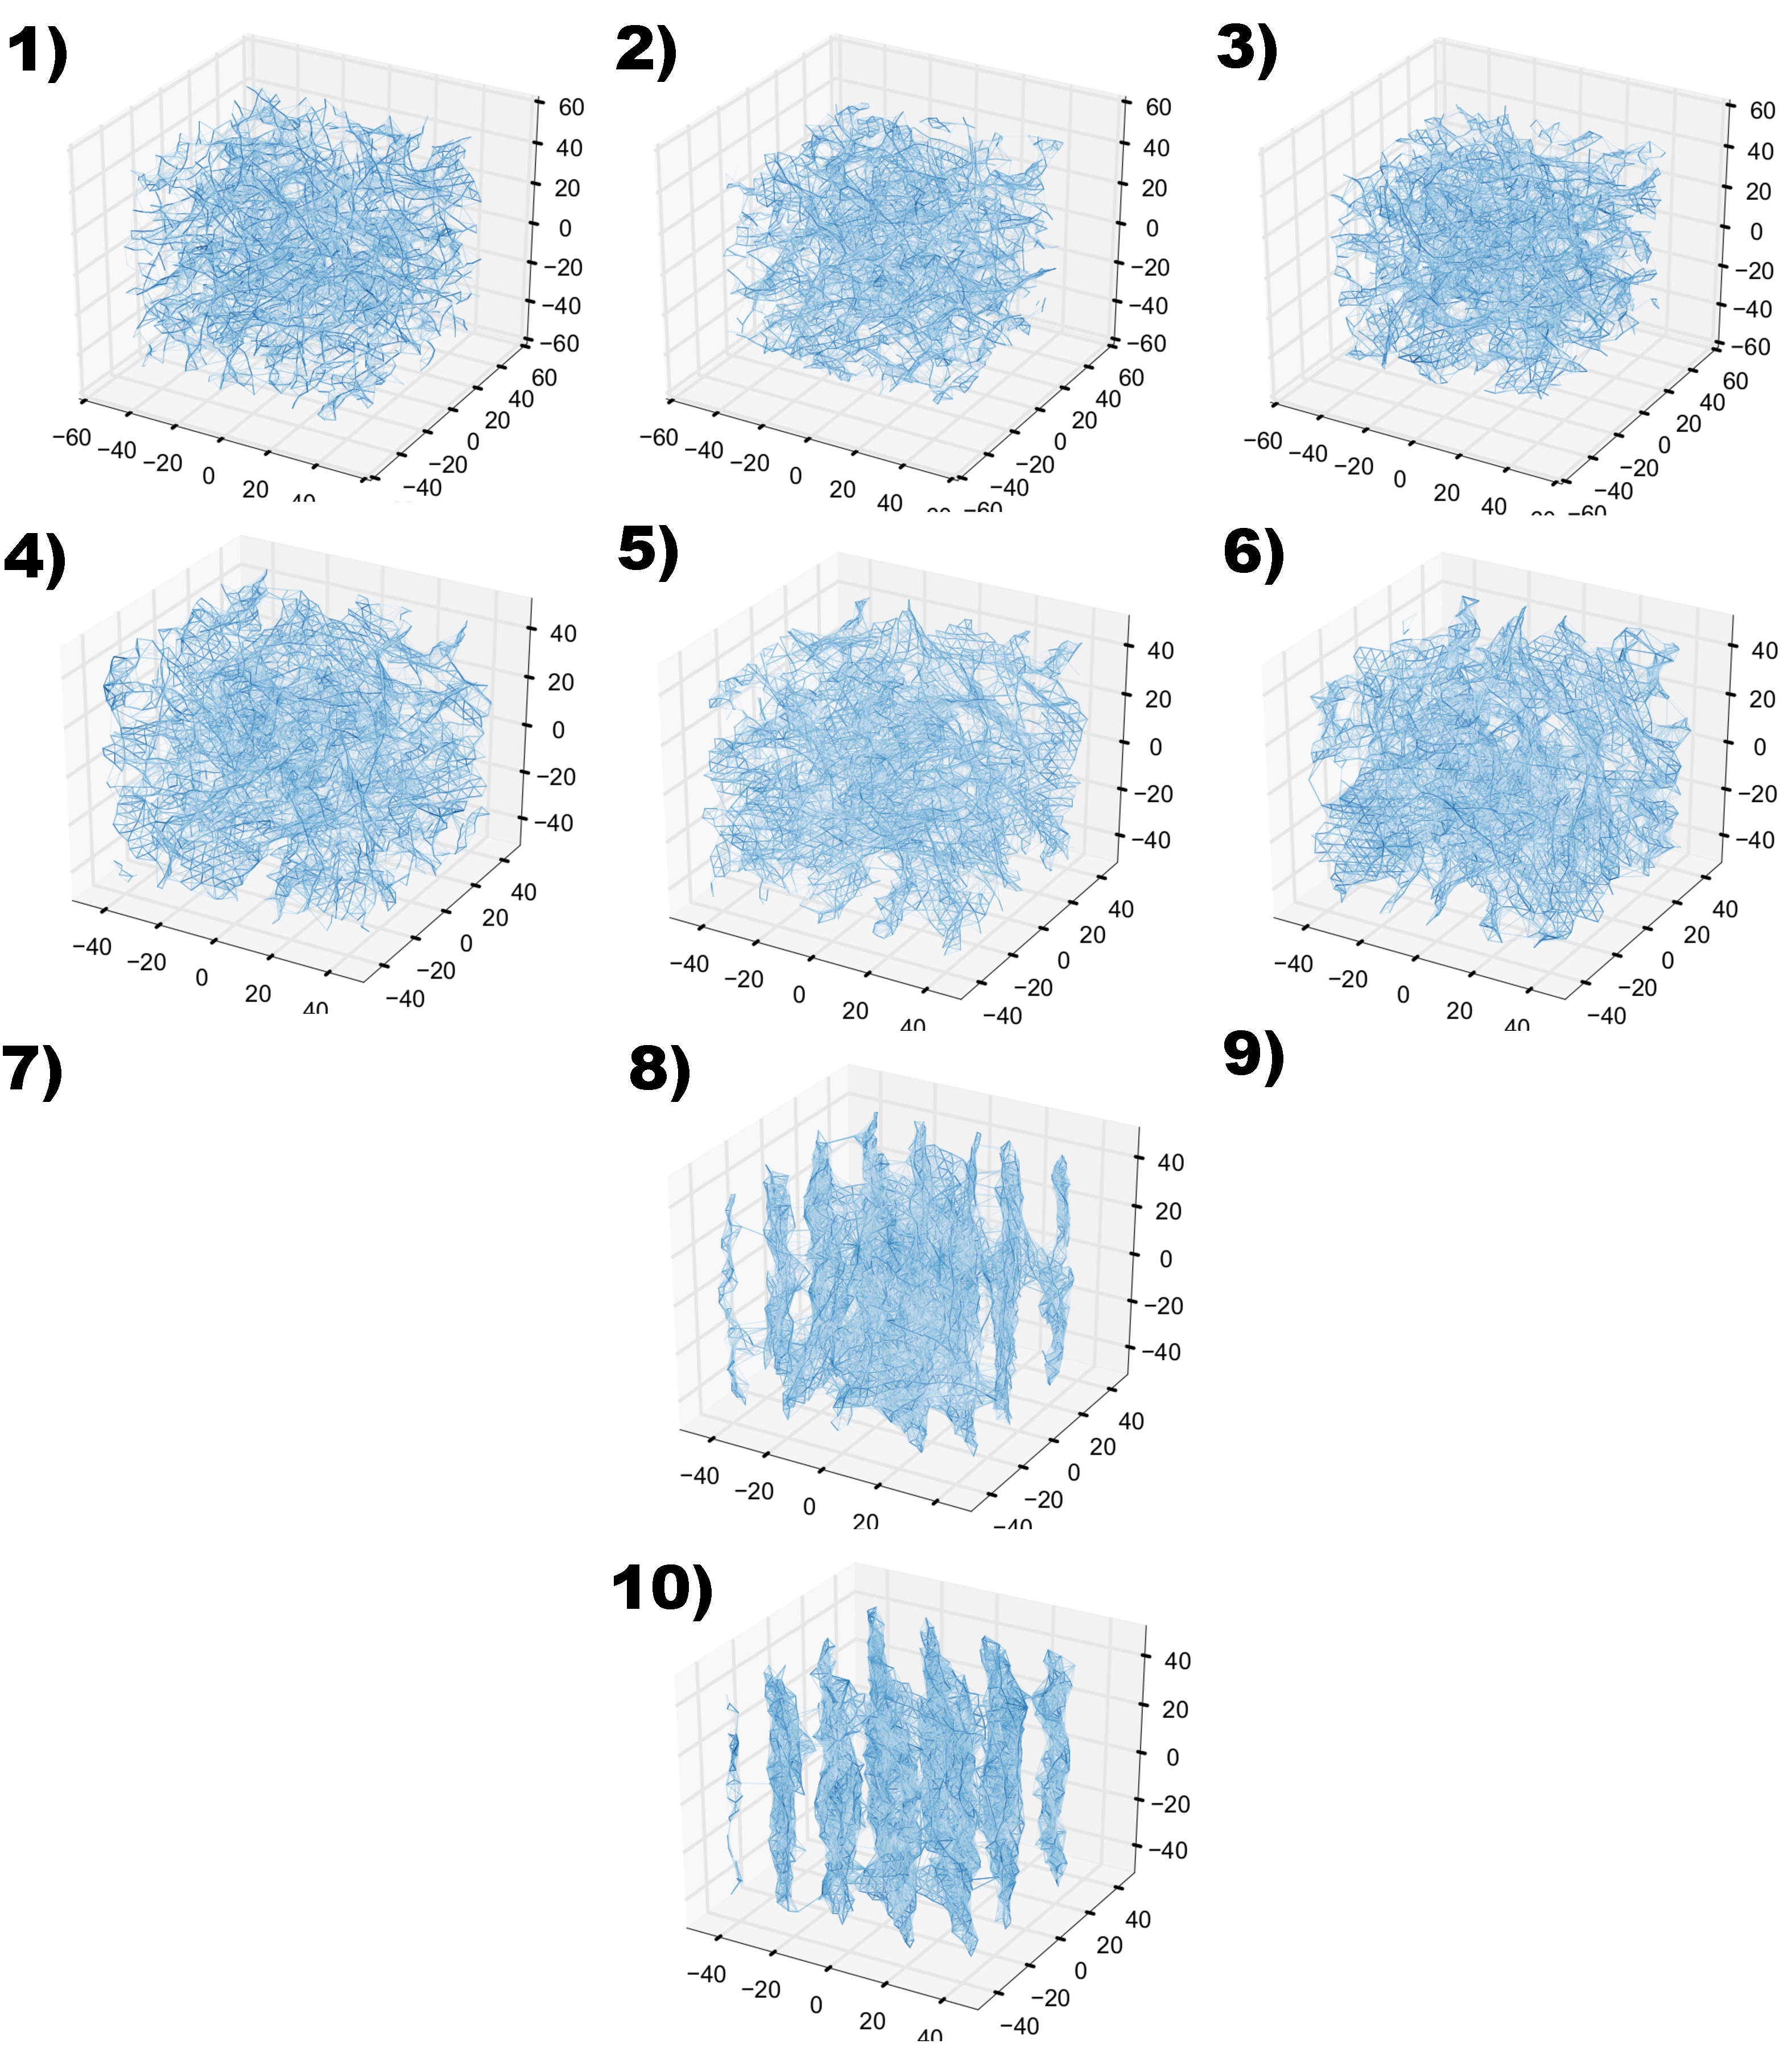
\includegraphics[width=\textwidth]{Figures/3dHole.pdf}
    \caption{The 3D heatmap of charge transport routes within the morphologies \textbf{1} - \textbf{10}.
    Dark routes describe commonly accessed hops between pairs of chromophores, whereas pale routes are less widely used in the KMC simulations.
    Each node therefore represents the location of a single chromophore.
The intensity value for the route is currently taken to be \texttt{I $=$ np.log10(freq) $/$ np.log10(max\_freq)}.}
	\label{fig:3dNetwork}
\end{figure}

\clearpage
\subsection{Anisotropies}


\begin{figure}[h!]\centering
	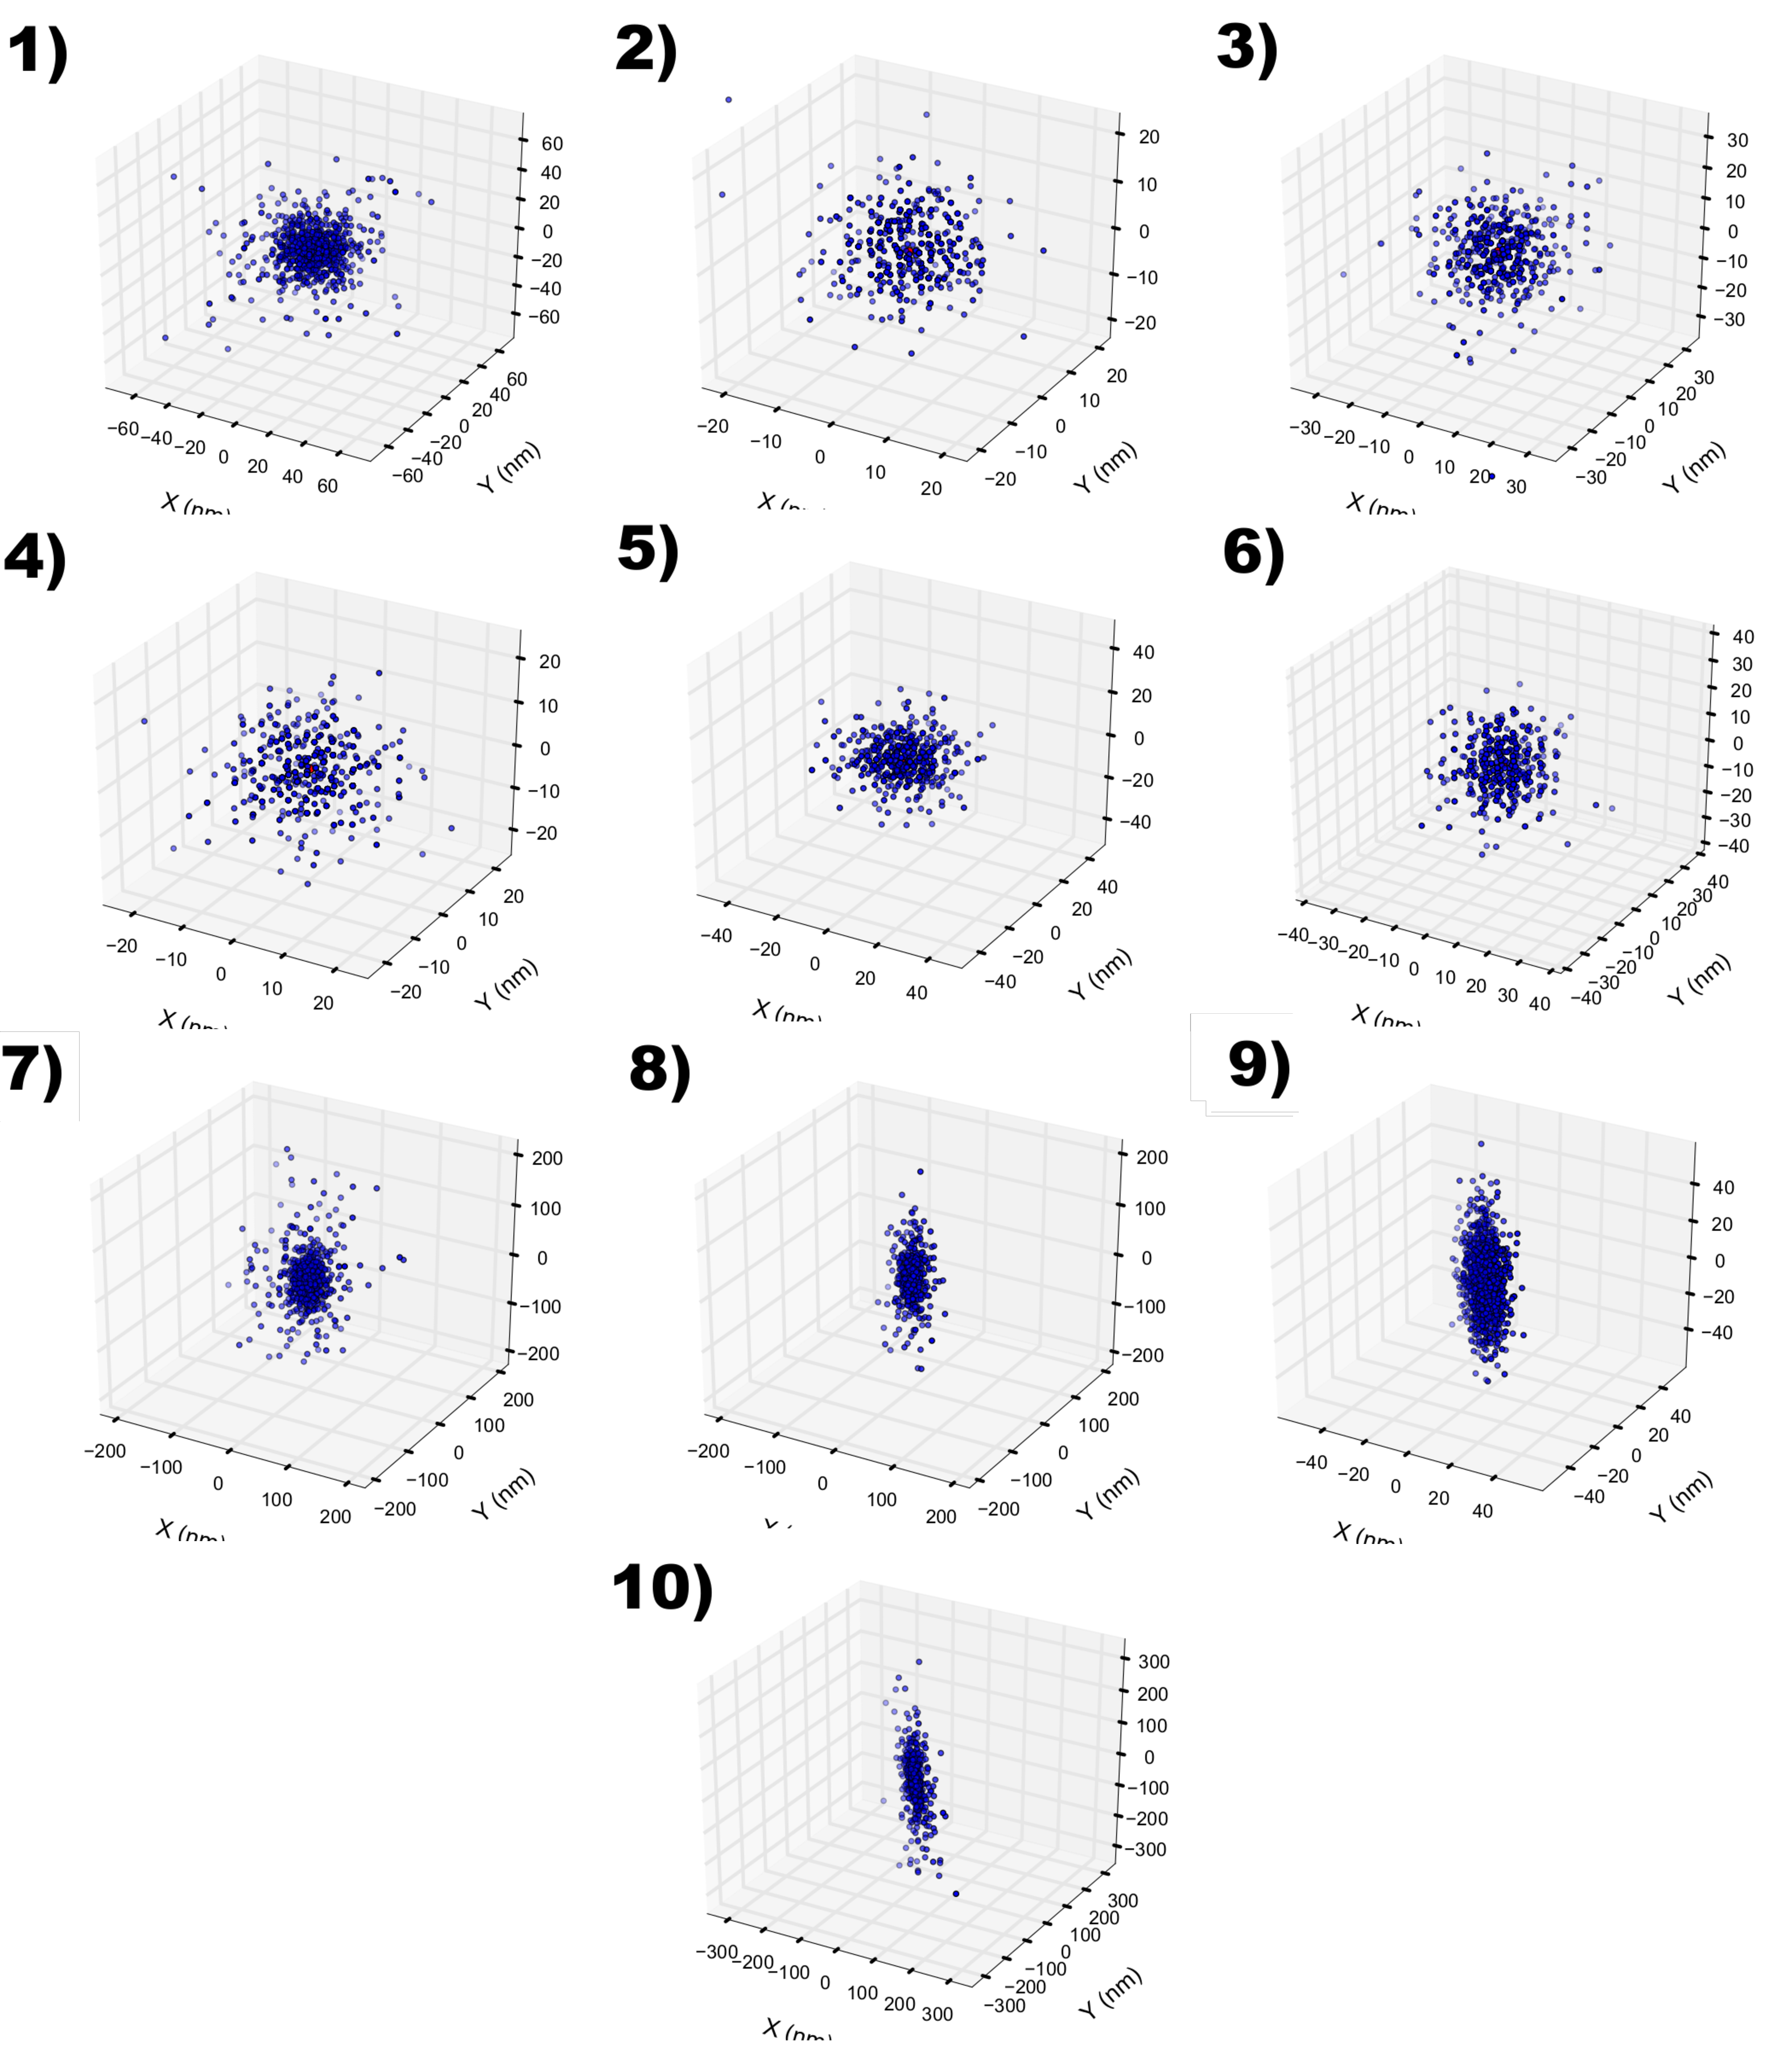
\includegraphics[width=\textwidth]{Figures/3dAnisotropy.pdf}
    \caption{The periodic anistropies of the carrier transport within the morphologies \textbf{1} - \textbf{10}.}
	\label{fig:MSD}
\end{figure}

\clearpage
\subsection{MSDs}


\begin{figure}[h!]\centering
	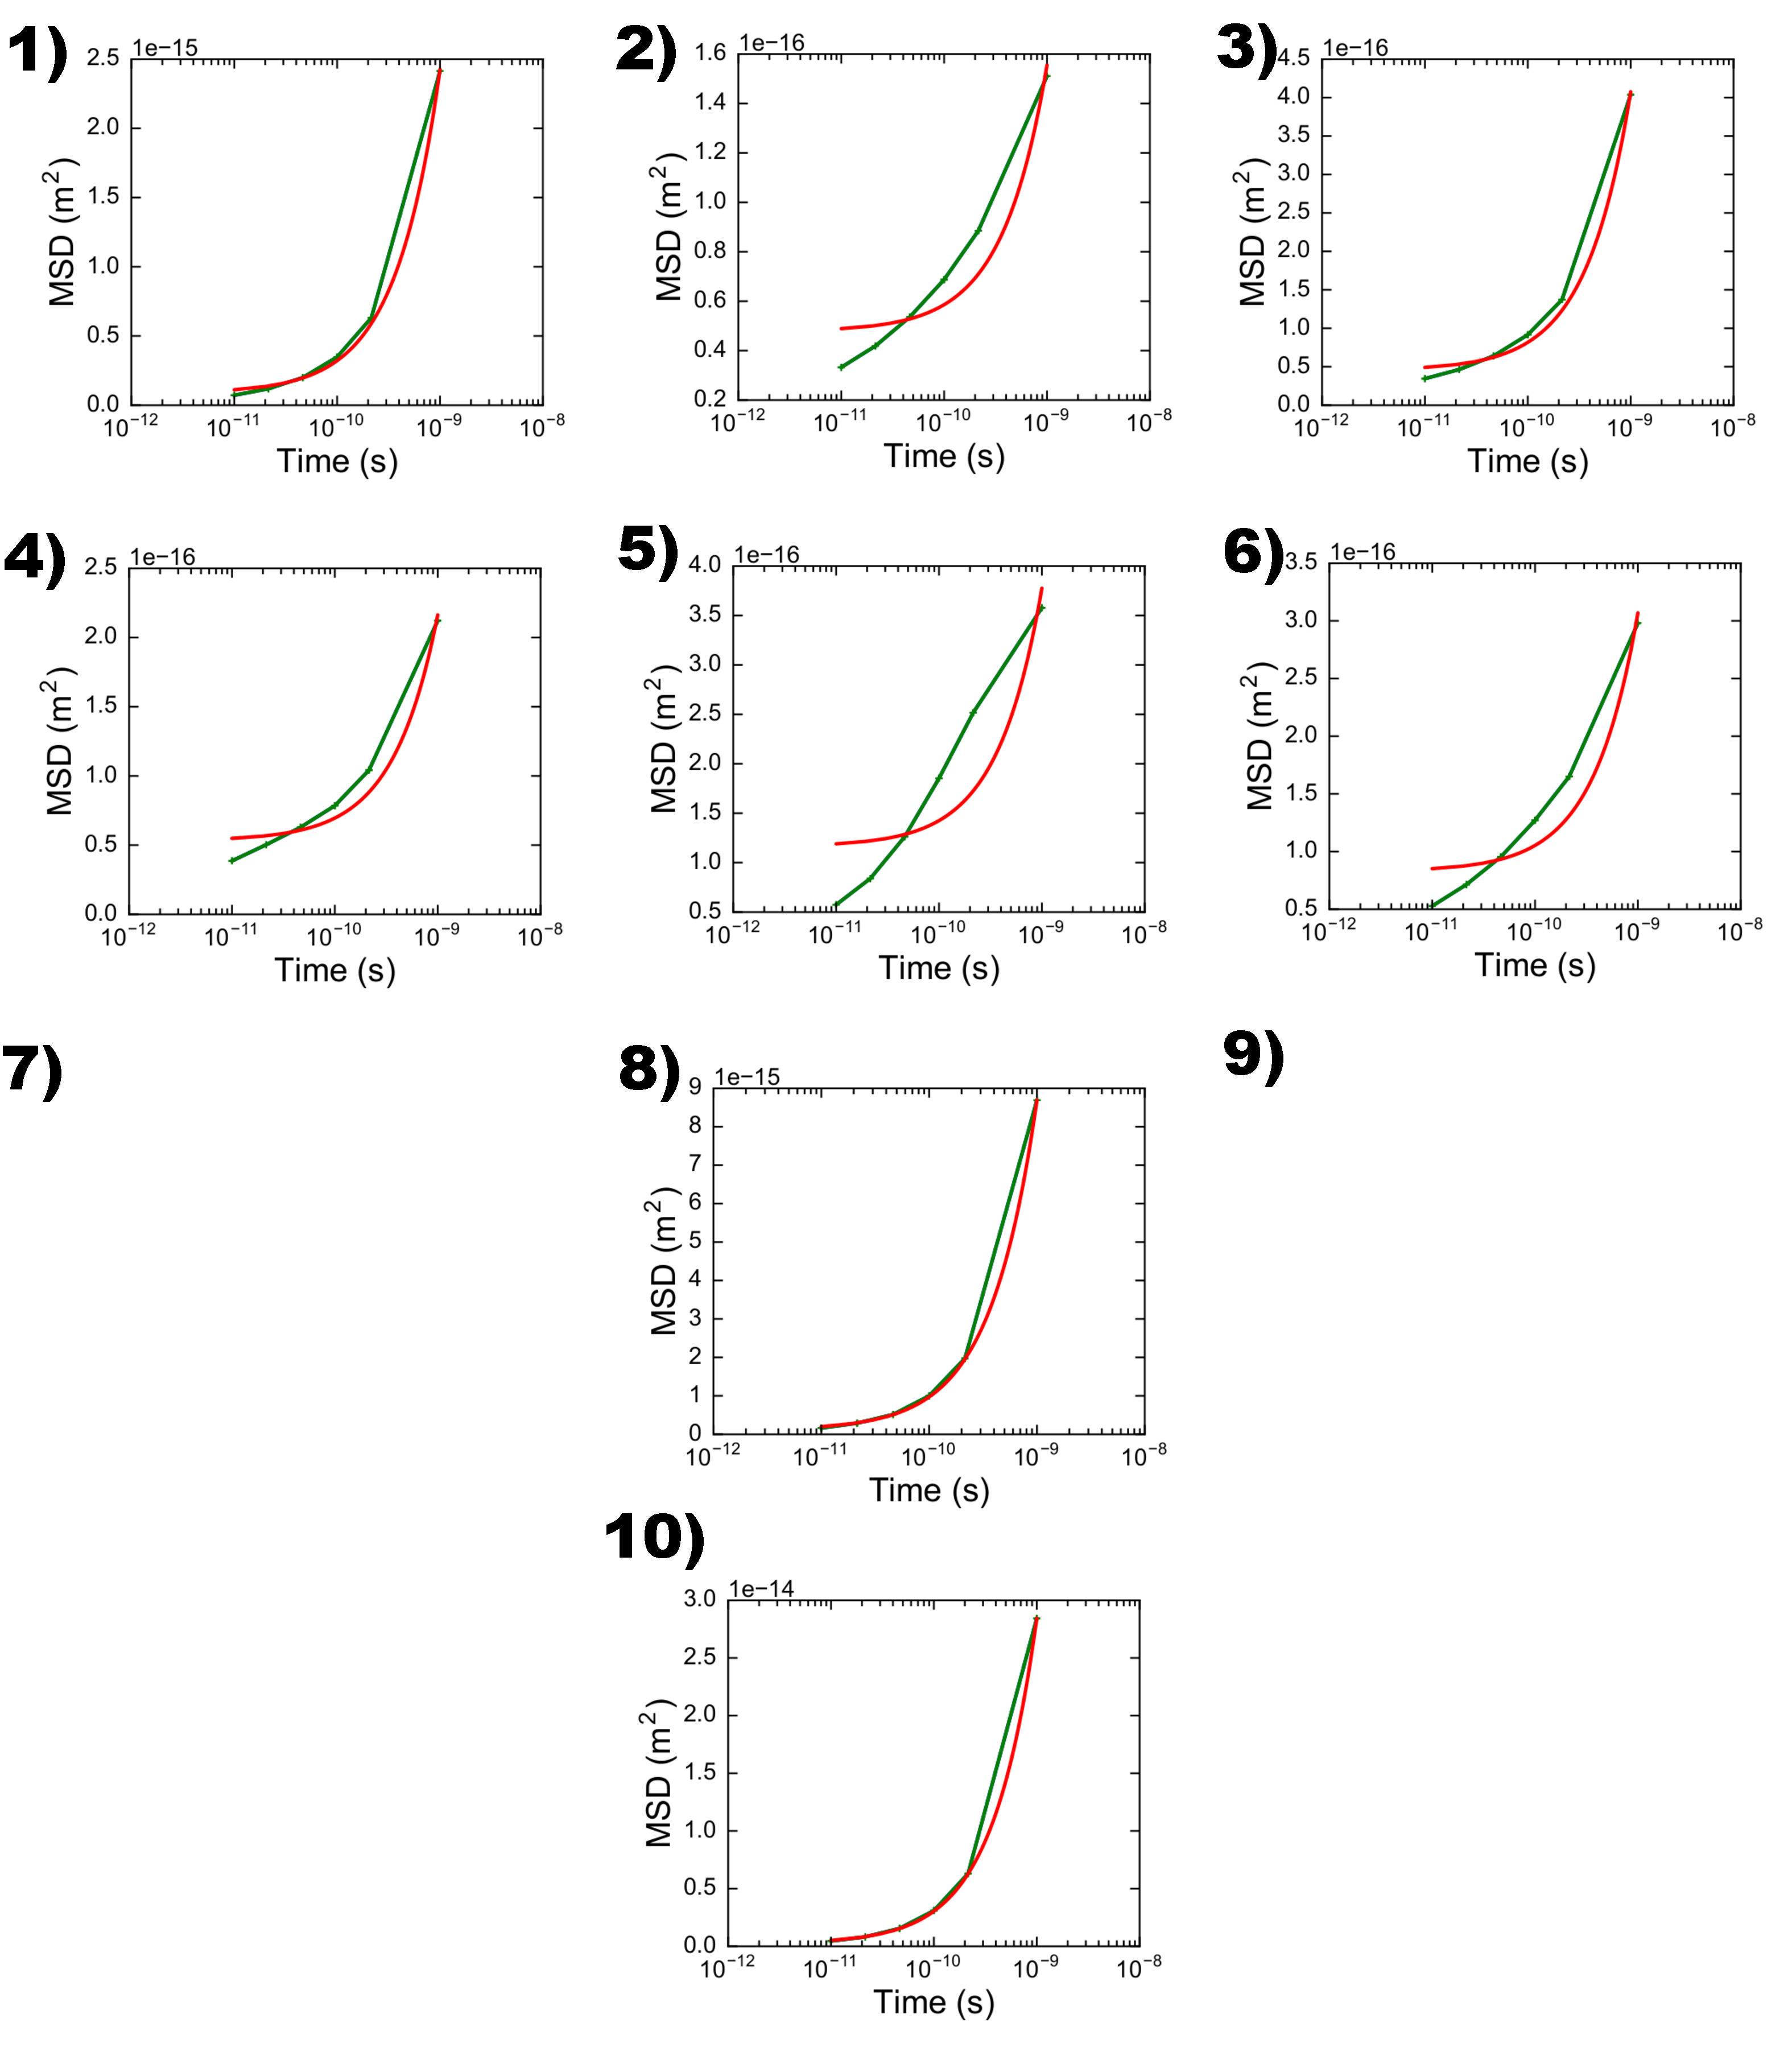
\includegraphics[width=\textwidth]{Figures/MSDs.pdf}
    \caption{The semi-log-x mean squared displacement curves of the carriers within the morphologies \textbf{1} - \textbf{10}.}
	\label{fig:MSD}
\end{figure}


\clearpage
\subsection{Hopping Rate Distributions}

\begin{figure}[h!]\centering
	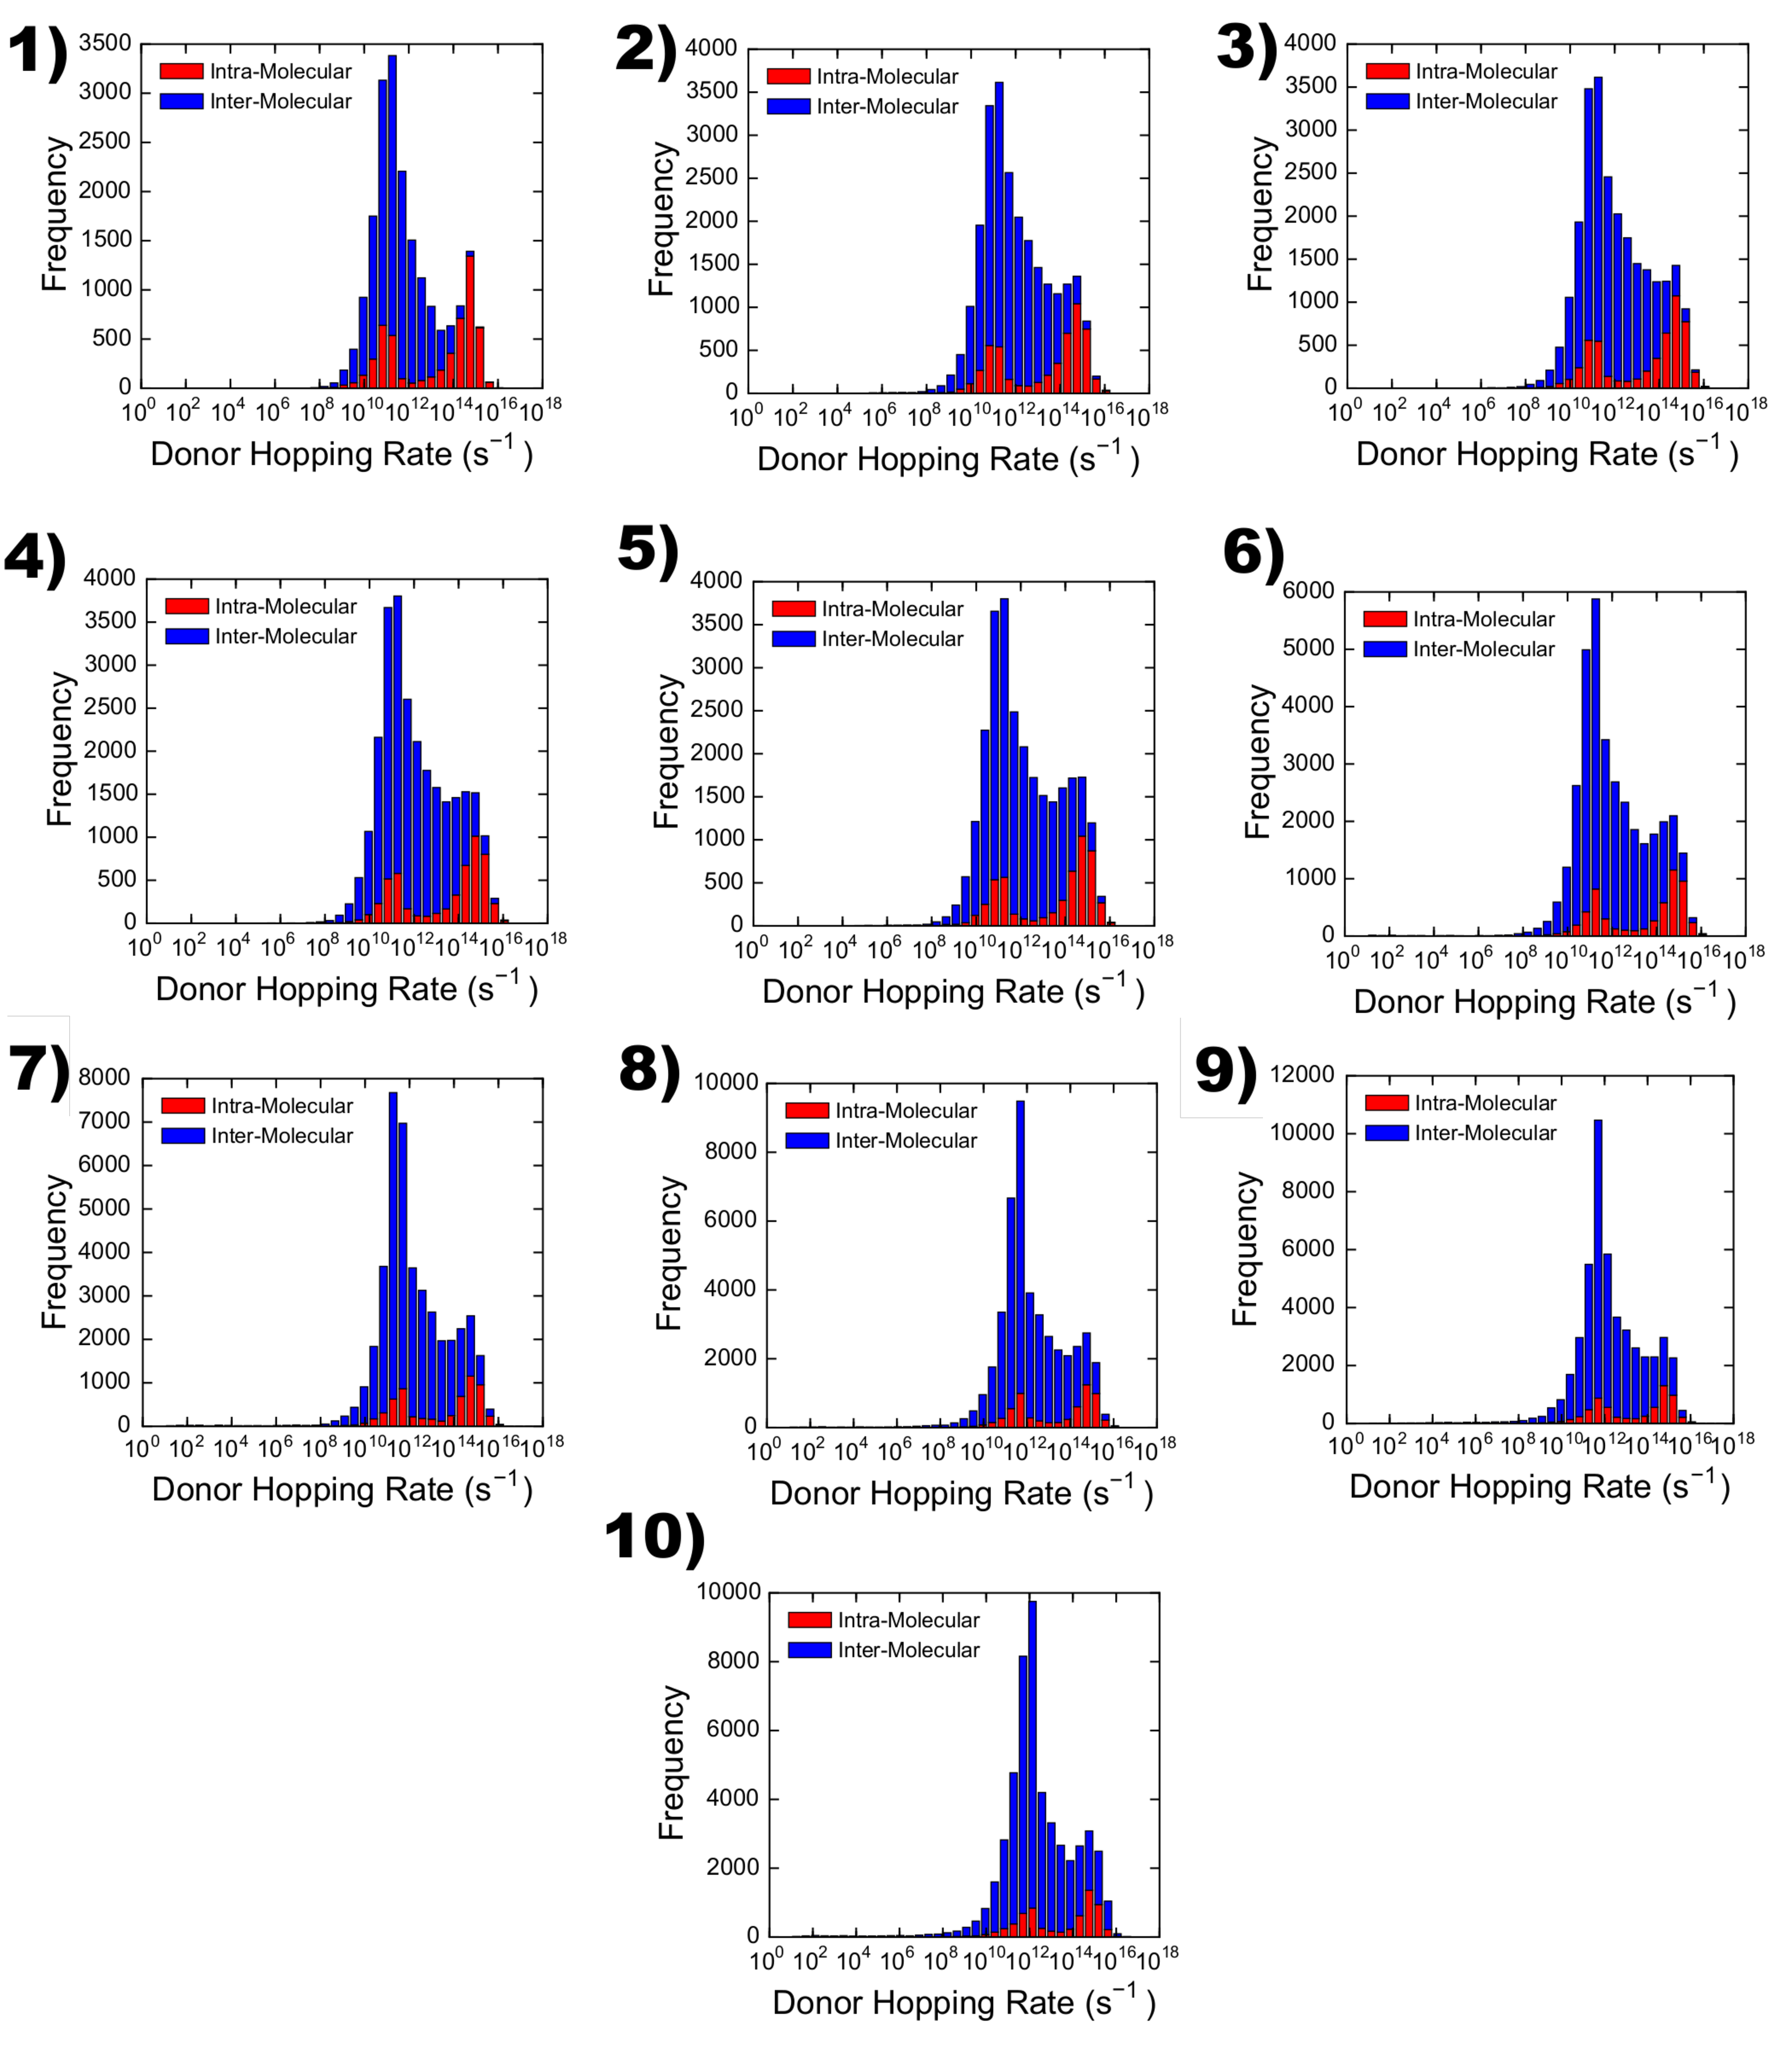
\includegraphics[width=\textwidth]{Figures/HoppingRates.pdf}
    \caption{The stacked hopping-rate distributions for intra- and inter-molecular hops executed by carriers within the morphologies \textbf{1} - \textbf{10}.}
	\label{fig:HoppingRateMixed}
\end{figure}

\clearpage


\bibliography{refs}
\bibliographystyle{unsrt}


\end{document}
